% Provenance (never printed): enseignement scientifique premiere (2019),
% "Le Soleil, notre source d'energie" (power received by latitude and
% season, albedo, the Earth's radiative balance, the small share stored by
% photosynthesis) and the old seconde/premiere S material on the
% atmosphere's energy; see sources/book2/PROVENANCE.md. Every insolation
% value, budget closure and photosynthesis figure is computed in
% figdata/grade-10/energy_budget.py; the budget fluxes are AR6 WG1
% Figure 7.2.
\chapter{Le bilan énergétique de la Terre}\label{ch:g10:earth-energy-budget}

Le jour le plus long de l'année, le Soleil ne se couche pas au pôle Nord. Il
tourne toute la journée dans le ciel à la même hauteur, environ
\qty{23}{\degree} au-dessus de l'horizon, et le sommet de l'atmosphère
au-dessus du pôle reçoit en un jour plus de lumière solaire par mètre carré
que partout ailleurs sur la Terre --- \qty{13.0}{kWh}, contre \qty{9.5}{kWh}
au-dessus de l'équateur. Pourtant, la mer autour du pôle reste couverte de
glace tout l'été. Sur une année entière, en revanche, l'équateur reçoit deux
fois et demie plus de lumière solaire que le pôle, et les tropiques restent
chauds toute l'année. Ce chapitre suit l'énergie de la lumière solaire~:
combien en arrive, où et quand~; combien est renvoyée directement vers
l'espace~; comment le reste se partage entre l'air et le sol, est transporté
des tropiques vers les pôles, puis renvoyé enfin vers l'espace sous forme
d'infrarouge --- et quelle part infime finit stockée par les êtres vivants.
% ledger: earth:TSI, earth:obliquity (daily totals computed in figdata/grade-10/energy_budget.py)

\begin{omfigure}
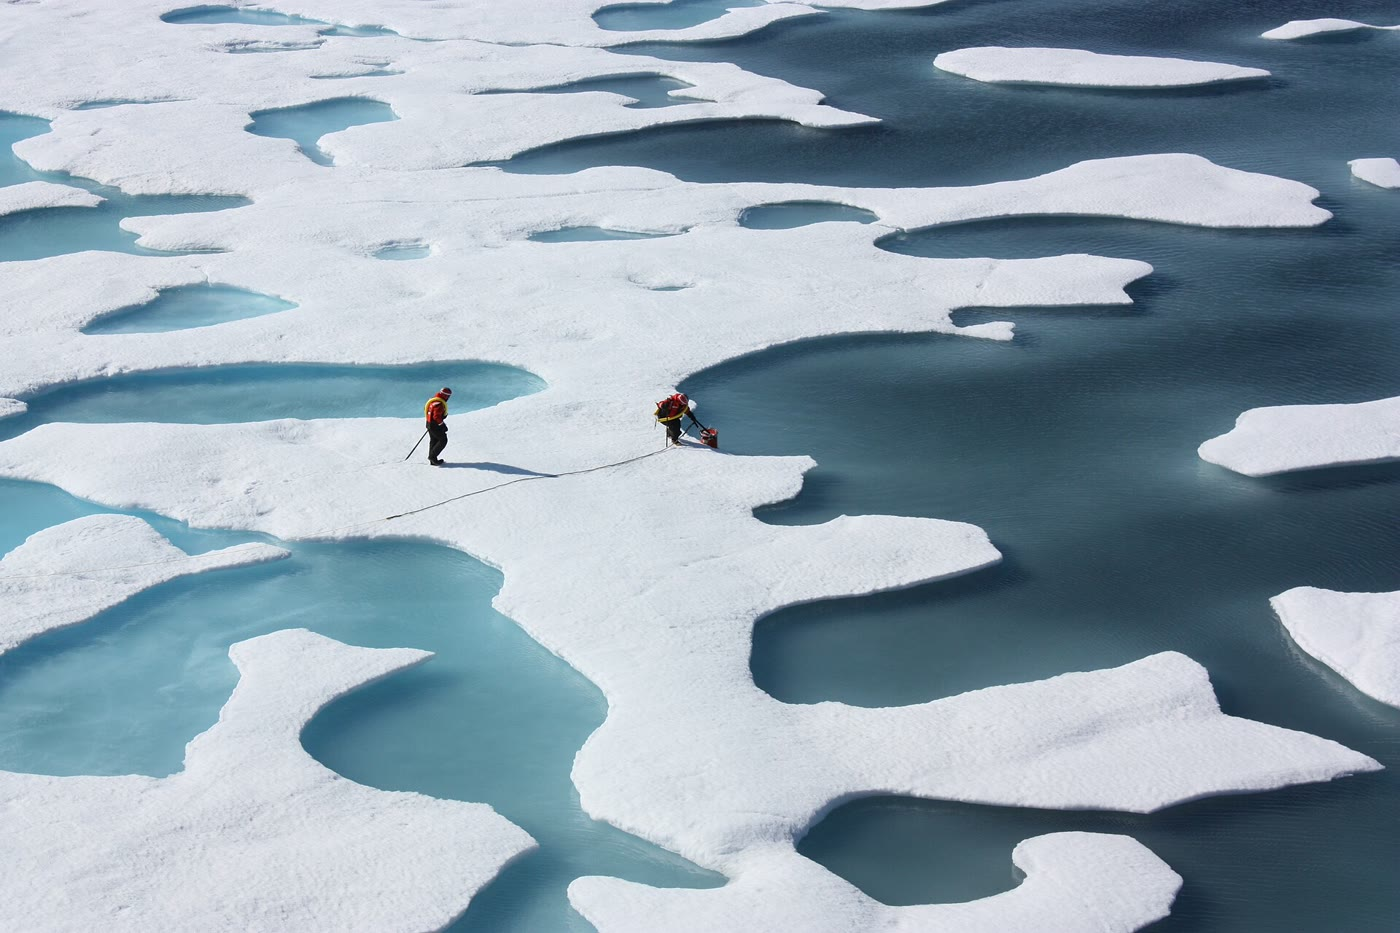
\includegraphics[width=0.78\linewidth]{images/book2/g10-nasa-melt-ponds.jpg}

{\small La banquise de l'océan Arctique en juillet, sous un Soleil qui ne se
couche pas~: de la glace blanche, des mares de fonte à sa surface, et la mer
libre, sombre, entre les plaques de glace. Deux scientifiques prélèvent de
l'eau des mares. Photographie~: NASA Goddard Space Flight Center, 2011
(domaine public).}
\end{omfigure}

\begin{recall}
Les saisons viennent de l'inclinaison de l'axe de la Terre,
\qty{23.44}{\degree} par rapport à la perpendiculaire au plan de son
orbite~: en juin, l'hémisphère Nord penche vers le Soleil, qui monte plus
haut dans son ciel et reste plus longtemps levé (les livres de physique, et
le livre~1). L'éclairement à la distance de la Terre,
$S_0 = \qty{1361}{W/m^2}$, l'\omterm{def:g10:earth-energy-budget:albedo}{albédo} de Bond d'une planète et sa \omterm{def:g10:habitable-planet:equilibrium-temperature}{température
d'équilibre} ont été vus au \cref{ch:g10:habitable-planet}. Les gaz à effet
de serre absorbent une partie de l'infrarouge émis par la surface (les
livres de chimie). L'air chaud monte et l'air froid descend, ce qui fait
tourner l'air en cellules de convection et entraîne les vents de la
circulation générale (livre~1, année~8). Les plantes, les algues et
certaines bactéries fabriquent des sucres à partir de dioxyde de carbone et
d'eau grâce à l'énergie de la lumière~: c'est la photosynthèse (les livres
de biologie).
\end{recall}

\section{La lumière solaire reçue}

Vue du Soleil, la Terre est un disque. À chaque seconde, elle intercepte la
lumière solaire qui tombe sur un disque de rayon $R$, son propre rayon~;
mais cette lumière se partage entre tous les points d'une sphère, dont la
moitié est dans la nuit.

\begin{proposition}[Le quart de la constante solaire]\label{prop:g10:earth-energy-budget:quarter}
En moyenne sur toute la surface de la Terre, de jour comme de nuit, la
puissance de la lumière solaire qui arrive au sommet de l'atmosphère vaut
\[
  \frac{S_0}{4} = \frac{1361}{4} \approx \qty{340}{W/m^2}.
\]
\end{proposition}

\begin{proof}
La Terre intercepte la lumière solaire qui traverse un disque d'aire
$\pi R^2$ perpendiculaire aux rayons, soit une puissance $S_0\,\pi R^2$.
Répartie sur l'aire de la sphère, $4\pi R^2$, elle donne $S_0\,\pi R^2/(4\pi R^2) =
S_0/4$ par mètre carré.
\end{proof}
% ledger: earth:TSI, ipcc:budget-toa

\begin{omfigure}
\begin{tikzpicture}[font=\small, >={Stealth[length=2mm]}]
  \foreach \y in {-1.2,-0.8,...,1.21}
    \draw[->, omProp!80!black] (-3.4,\y) -- (-1.75,\y);
  \node[anchor=south, font=\footnotesize, align=center] at (-2.6,1.35) {lumière solaire,\\$S_0$ par m$^2$};
  \draw[fill=omProp!15, draw=omProp!80!black] (-1.6,0) ellipse (0.18 and 1.3);
  \node[anchor=north, font=\footnotesize, align=center] at (-1.6,-1.4) {disque\\$\pi R^2$};
  \shade[ball color=omDef!35] (1.2,0) circle (1.3);
  \fill[black, opacity=0.35] (1.2,1.3) arc (90:-90:1.3) arc (-90:90:0.35 and 1.3);
  \draw[omDef!80!black] (1.2,0) circle (1.3);
  \draw[dashed, black!50] (1.2,-1.3) arc (-90:90:0.35 and 1.3);
  \draw[<->] (1.2,0) -- node[above, font=\footnotesize] {$R$} (2.5,0);
  \node[anchor=west, font=\footnotesize, align=left] at (2.8,0.7) {sphère $4\pi R^2$~:\\moitié au jour,\\moitié dans la nuit};
  \node[anchor=west, font=\footnotesize, align=left] at (2.8,-0.75) {en moyenne~:\\$S_0\pi R^2/4\pi R^2 = S_0/4$};
\end{tikzpicture}

{\small La Terre intercepte la lumière solaire qui tombe sur un disque de
son propre rayon, mais la répartit sur l'aire quatre fois plus grande d'une
sphère~: en moyenne, chaque mètre carré du sommet de l'atmosphère reçoit le
quart de la constante solaire.}
\end{omfigure}

La moyenne cache de grandes différences d'un lieu à l'autre. Un faisceau de
lumière solaire qui frappe le sol en oblique se répartit sur une plus grande
surface qu'un faisceau qui le frappe de face.

\begin{proposition}[La lumière solaire sur une surface horizontale]\label{prop:g10:earth-energy-budget:height}
Lorsque le Soleil est à une hauteur $h$ au-dessus de l'horizon, un mètre
carré horizontal au sommet de l'atmosphère reçoit la puissance $S_0 \sin h$.
\end{proposition}

\begin{proof}
Prenons un faisceau de lumière solaire de section carrée de \qty{1}{m^2},
qui transporte $S_0$. Au sol, sa trace est un rectangle dont un côté mesure
\qty{1}{m} et l'autre une longueur $\ell$ dans le sens de la pente des
rayons. Dans le triangle rectangle formé par ce côté, le rayon et la section
du faisceau, l'angle au sol vaut $h$ et $\sin h = 1/\ell$. La puissance du
faisceau se répartit sur $\ell$ mètres carrés~: $S_0/\ell = S_0 \sin h$ par
mètre carré.
\end{proof}

\begin{omfigure}
\begin{tikzpicture}[font=\small, >={Stealth[length=2mm]}]
  \fill[omExo!15] (-0.3,-0.5) rectangle (6.3,0);
  \draw[thick] (-0.3,0) -- (6.3,0);
  \foreach \s in {0,0.3,...,1.21}
    \draw[->, omProp!80!black] ({0.6+\s/sin(35)+3.2*cos(35)},{3.2*sin(35)}) -- ({0.6+\s/sin(35)+0.02*cos(35)},{0.02*sin(35)});
  \draw[omProp!80!black, thick] (0.6,0) -- ({0.6+1.2/sin(35)},0);
  \draw (0.6,0) ++(1.6,0) arc (0:35:1.6);
  \node[font=\footnotesize] at ({0.6+1.85*cos(17)},{1.85*sin(17)}) {$h$};
  \draw[<->] (0.6,-0.25) -- node[below, font=\footnotesize] {$\ell = 1/\sin h$} ({0.6+1.2/sin(35)},-0.25);
  \node[anchor=south west, font=\footnotesize, align=left] at (4.35,1.95) {faisceau de\\section\\\qty{1}{m^2}};
\end{tikzpicture}

{\small Lumière solaire arrivant à une hauteur $h$ au-dessus de l'horizon~:
le même faisceau couvre $1/\sin h$ mètres carrés de sol horizontal, donc
chaque mètre carré reçoit $S_0 \sin h$. Plus le Soleil est bas, plus la
lumière solaire est faible au sol.}
\end{omfigure}

La hauteur du Soleil varie au cours de la journée, et la durée du jour
varie avec les saisons~; les deux comptent dans l'énergie que reçoit un
lieu.

\begin{definition}[Insolation]\label{def:g10:earth-energy-budget:insolation}
L'\emph{insolation}\index{insolation} d'un lieu est la puissance de la
lumière solaire reçue par un mètre carré horizontal au sommet de
l'atmosphère, au-dessus de ce lieu. Moyennée sur les vingt-quatre heures
d'une journée, c'est l'\emph{insolation moyenne journalière}~; moyennée sur
une année, l'\emph{insolation moyenne annuelle}~; toutes deux se mesurent en
\unit{W/m^2}.
\end{definition}

Le calcul de la moyenne journalière demande la hauteur du Soleil à chaque
instant de la journée, ce qui fait appel à des mathématiques qui dépassent
ce livre~; c'est un ordinateur qui a tracé les courbes ci-dessous. Deux cas
sont simples. Sur l'équateur à un équinoxe, le Soleil se lève plein est,
passe au zénith à midi et se couche plein ouest douze heures plus tard~; en
moyenne sur vingt-quatre heures, cela donne
$S_0/\pi \approx \qty{433}{W/m^2}$ (admis). Au pôle Nord, le Soleil tourne
simplement dans le ciel à une hauteur constante, ce qu'utilise l'exemple
suivant.

\begin{example}[Le pôle en juin]\label{ex:g10:earth-energy-budget:pole}
% ledger: earth:TSI, earth:obliquity (values computed in figdata/grade-10/energy_budget.py)
Au solstice de juin, le Soleil reste toute la journée à \qty{23.44}{\degree}
au-dessus de l'horizon du pôle Nord. L'\omterm{def:g10:earth-energy-budget:insolation}{insolation} moyenne journalière y vaut
$1361
\times \sin 23.44^\circ \approx \qty{541}{W/m^2}$~; sur vingt-quatre
heures, cela fait $541 \times 24 \approx \qty{13000}{Wh}$, soit
\qty{13.0}{kWh} par mètre carré. Le même jour, l'équateur reçoit en moyenne
journalière \qty{397}{W/m^2}, soit \qty{9.5}{kWh} par mètre carré~: le
Soleil y monte plus haut à midi, mais il reste couché douze heures.
\end{example}

\begin{omfigure}
\begin{tikzpicture}
\begin{axis}[omrecord, width=0.92\linewidth, height=6.4cm, xmin=1, xmax=365,
  ymin=0, ymax=600, ylabel={insolation moyenne journalière (\unit{W/m^2})},
  xtick={1,32,60,91,121,152,182,213,244,274,305,335},
  xticklabels={J,F,M,A,M,J,J,A,S,O,N,D}, xlabel={mois},
  legend style={at={(0.5,1.02)}, anchor=south, legend columns=4, font=\footnotesize, draw=none},
  tick label style={font=\small}, label style={font=\small}]
\addplot[omThm!85!black, thick] table[x=day, y=Q0] {figdata/out/grade-10-energy_budget-daily.dat};
\addlegendentry{équateur}
\addplot[omProp!90!black, thick, densely dashed] table[x=day, y=Q30] {figdata/out/grade-10-energy_budget-daily.dat};
\addlegendentry{\qty{30}{\degree} N}
\addplot[omMeth!85!black, thick, dashdotted] table[x=day, y=Q60] {figdata/out/grade-10-energy_budget-daily.dat};
\addlegendentry{\qty{60}{\degree} N}
\addplot[omDef!85!black, thick] table[x=day, y=Q90] {figdata/out/grade-10-energy_budget-daily.dat};
\addlegendentry{pôle Nord}
\end{axis}
\end{tikzpicture}

{\small \omterm{def:g10:earth-energy-budget:insolation}{Insolation} moyenne journalière au sommet de l'atmosphère au cours de
l'année, à quatre latitudes de l'hémisphère Nord (calculée pour une orbite
circulaire, à partir de la constante solaire et de l'inclinaison de l'axe).
Le pôle ne reçoit rien pendant la moitié de l'année, et plus que tout autre
lieu autour du solstice de juin.}
\end{omfigure}

\begin{remark}[Lire les courbes]\label{rem:g10:earth-energy-budget:curves}
L'\omterm{def:g10:earth-energy-budget:insolation}{insolation} de l'équateur varie à peine~: deux maximums peu marqués aux
équinoxes, quand le Soleil passe au zénith à midi. Plus on va vers le nord,
plus l'écart entre l'été et l'hiver est grand. Au-delà de
$90^\circ - 23.44^\circ = \qty{66.56}{\degree}$, le Soleil reste sous
l'horizon au solstice de décembre~: c'est la nuit polaire. D'environ le
10~mai à la fin juillet, le pôle Nord et la latitude \qty{60}{\degree} N
reçoivent tous deux plus que l'équateur.
\end{remark}

Sur une année entière, le tableau change~: l'\omterm{def:g10:earth-energy-budget:insolation}{insolation} moyenne annuelle,
représentée dans la section sur l'excédent et le déficit ci-dessous, passe
de \qty{416}{W/m^2} à l'équateur à \qty{172}{W/m^2} aux pôles. L'abondance
estivale des régions polaires ne compense pas leur longue nuit et leur
Soleil bas.

\begin{remark}[La distance au Soleil ne fait pas les saisons]\label{rem:g10:earth-energy-budget:distance}
% ledger: earth:peri, earth:aph, nasa:earth-perihelion-longitude (ratios computed)
L'orbite de la Terre n'est pas tout à fait un cercle~: sa distance au
Soleil varie entre \num{147.1} et \num{152.1} millions de kilomètres,
d'environ \qty{3}{\percent}, si bien que la lumière solaire reçue varie
d'environ \qty{7}{\percent}. La Terre est au plus près du Soleil début
janvier, au cœur de l'hiver boréal. Les courbes ci-dessus négligent ce
faible écart~; les saisons viennent de l'inclinaison de l'axe, et elles
sont inversées dans les deux hémisphères.
\end{remark}

\section{L'albédo}

Une partie de la lumière solaire qui atteint la Terre ne réchauffe jamais
rien~: les nuages, l'air, la neige et la mer la renvoient vers l'espace.

\begin{definition}[Albédo]\label{def:g10:earth-energy-budget:albedo}
L'\emph{albédo}\index{albedo@albédo} d'une surface est la fraction de la
lumière solaire incidente qu'elle réfléchit, un nombre compris entre 0
(toute la lumière est absorbée) et 1 (toute la lumière est réfléchie).
L'albédo de Bond du \cref{ch:g10:habitable-planet} est l'albédo d'une
planète prise dans son ensemble.
\end{definition}

\begin{omfigure}
\begin{tikzpicture}[font=\small, x=9cm, y=0.55cm]
  \foreach \lab/\lo/\hi/\n in {neige fraîche/0.80/0.90/8, banquise/0.50/0.70/7,
      sable du désert/0.40/0.40/6, Terre entière/0.30/0.30/5, herbe verte/0.25/0.25/4,
      sol nu/0.17/0.17/3, forêt de conifères/0.08/0.15/2, océan libre/0.06/0.06/1,
      asphalte neuf/0.04/0.04/0} {
    \fill[omDef!45] (0,\n-0.32) rectangle (\lo,\n+0.32);
    \ifdim\hi pt>\lo pt
      \fill[omDef!18] (\lo,\n-0.32) rectangle (\hi,\n+0.32);
      \draw[omDef!80!black] (\lo,\n-0.32) rectangle (\hi,\n+0.32);
    \fi
    \draw[omDef!80!black] (0,\n-0.32) rectangle (\lo,\n+0.32);
    \node[anchor=east, font=\footnotesize] at (-0.01,\n) {\lab};
  }
  \draw (0,-0.6) -- (1,-0.6);
  \foreach \x in {0,0.2,...,1.01}
    \draw (\x,-0.6) -- (\x,-0.75) node[below, font=\footnotesize] {\pgfmathprintnumber[fixed, precision=1]{\x}};
  \node[font=\footnotesize] at (0.5,-2.0) {albédo};
\end{tikzpicture}

{\small \omterm{def:g10:earth-energy-budget:albedo}{Albédos} typiques de surfaces et de la Terre dans son ensemble~; la
partie claire d'une barre indique l'intervalle habituel. Données~:
université du Colorado à Boulder, expédition MOSAiC~; National Snow and Ice
Data Center.}
\end{omfigure}
% ledger: albedo:surfaces, nsidc:albedo-ice

La neige fraîche renvoie l'essentiel de la lumière qu'elle reçoit, l'océan
libre presque rien. C'est pourquoi la banquise de la photographie
d'ouverture garde son froid pendant l'été polaire~: la neige qui la recouvre
réfléchit jusqu'aux neuf dixièmes de la lumière solaire, tandis que l'eau
sombre entre les plaques de glace en absorbe environ 94 pour cent. Quand la
glace fond, l'eau sombre la remplace et absorbe davantage de lumière
solaire, ce qui fait fondre plus de glace~: une boucle qui se renforce
elle-même, que le \cref{ch:g12:climate-change} évalue parmi les
rétroactions du climat.

\begin{omfigure}
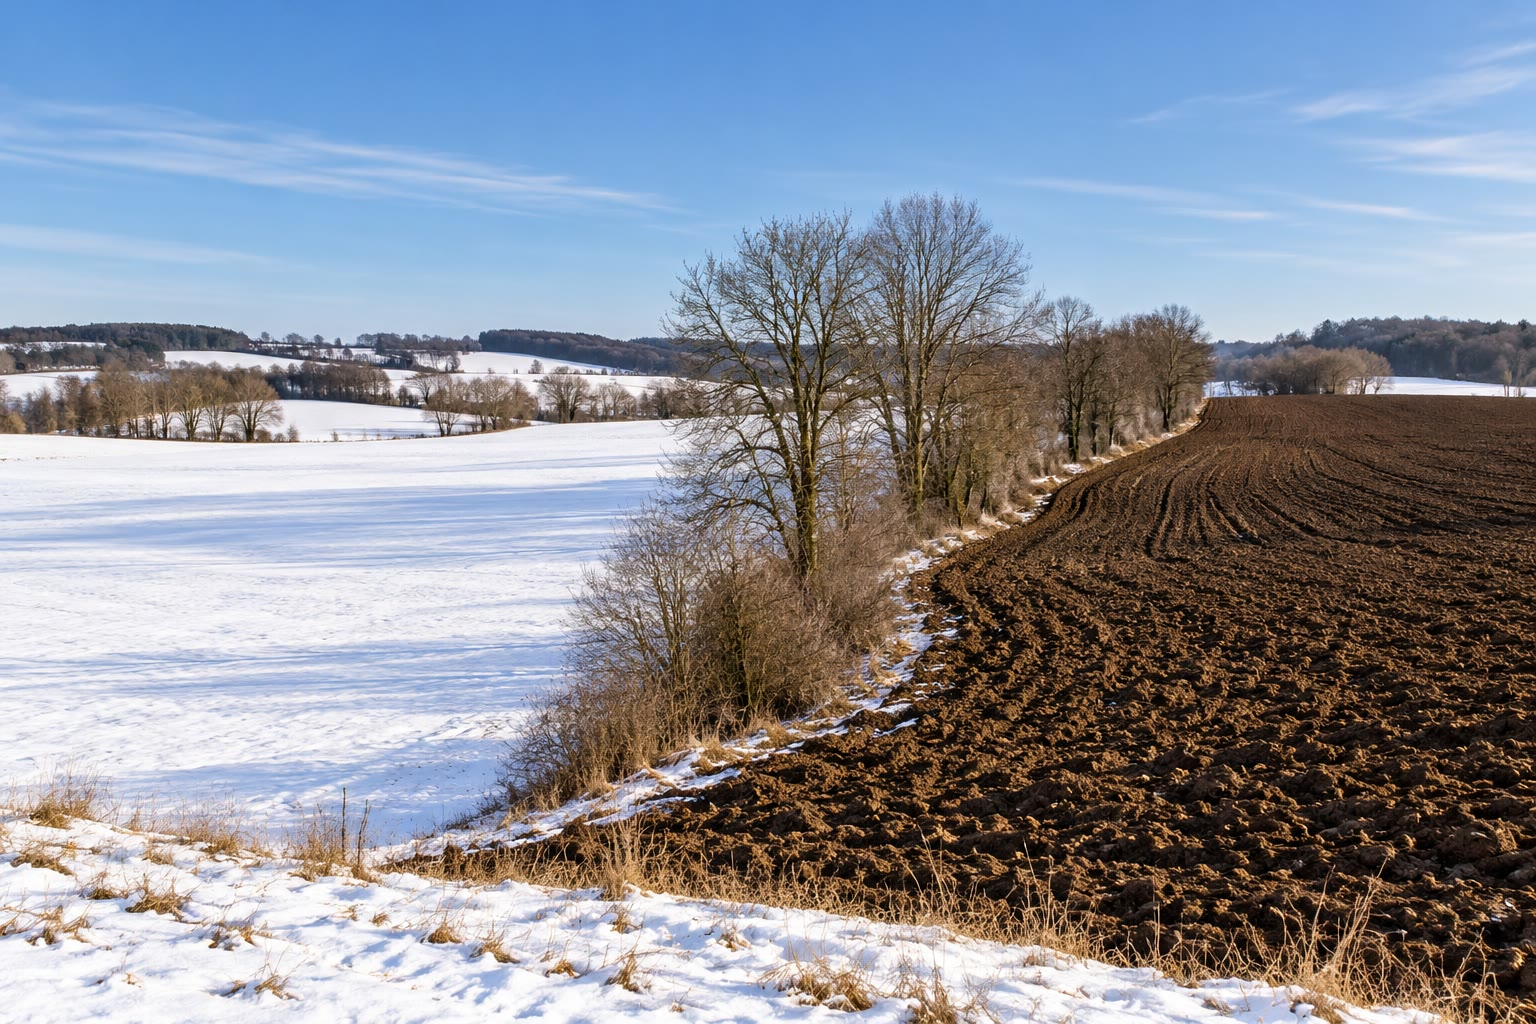
\includegraphics[width=0.7\linewidth]{images/book2/ai/g10-snow-and-ploughed-field.jpg}

{\small Un matin d'hiver après quelques jours de soleil~: la neige recouvre
encore le pré, mais elle a fondu sur le champ labouré sombre, qui absorbe
beaucoup plus de lumière solaire.}
\end{omfigure}

Pour la Terre dans son ensemble, les satellites mesurent directement la
lumière solaire réfléchie vers l'espace~: en moyenne \qty{100}{W/m^2} sur
les \qty{340}{W/m^2} qui arrivent, soit un \omterm{def:g10:earth-energy-budget:albedo}{albédo} de $100/340 \approx 0.29$.
Les nuages sont le principal réflecteur~: les mêmes mesures, nuages
retranchés par le calcul, ne donnent que \qty{53}{W/m^2} réfléchis.
% ledger: ipcc:budget-toa, ipcc:budget-clearsky, earth:albedo

\begin{example}[La lumière solaire absorbée par la Terre]\label{ex:g10:earth-energy-budget:absorbed}
% ledger: earth:TSI, earth:albedo, earth:Rmean (computed in figdata/grade-10/energy_budget.py)
Avec un \omterm{def:g10:earth-energy-budget:albedo}{albédo} de Bond de 0.294, chaque mètre carré absorbe en moyenne
$340
\times (1 - 0.294) \approx \qty{240}{W/m^2}$. Sur toute la sphère,
d'aire $4\pi R^2 = 4\pi \times (\qty{6.371e6}{m})^2 \approx \qty{5.10e14}{m^2}$,
la Terre absorbe $240 \times 5.10\times10^{14} \approx \qty{1.22e17}{W}$ de
lumière solaire~: c'est cette puissance qui entraîne les vents, les courants
océaniques et le cycle de l'eau.
\end{example}

\section{Le bilan énergétique global}

Où vont ces \qty{240}{W/m^2}~? Les mesures des satellites, des instruments
au sol et des navires, combinées à des modèles de l'atmosphère, donnent
aujourd'hui une réponse cohérente, en moyenne sur le globe et sur plusieurs
années. Le rapport d'évaluation scientifique de 2021 la résume dans le
schéma ci-dessous, et indique que les composantes moyennes globales sont
désormais connues avec plus de précision, au sommet de l'atmosphère comme à
la surface (\emph{degré de confiance élevé}).
% ledger: ipcc:budget-confidence

\begin{definition}[Bilan énergétique]\label{def:g10:earth-energy-budget:energy-budget}
Le \emph{bilan énergétique}\index{bilan energetique@bilan énergétique} d'un
système --- la Terre entière, sa surface ou son atmosphère --- est le compte
de toute l'énergie qui y entre et qui en sort, chaque flux étant donné comme
une puissance moyenne par mètre carré de surface terrestre. Le bilan est
\emph{équilibré} quand ce qui entre égale ce qui sort~; sinon, le système
gagne ou perd de l'énergie, et se réchauffe ou se refroidit.
\end{definition}

La surface perd aussi de l'énergie sans aucun rayonnement~: l'eau s'évapore
de la mer et des feuilles, et le sol réchauffe l'air à son contact.

\begin{definition}[Chaleur latente~; chaleur sensible]\label{def:g10:earth-energy-budget:latent-heat}
La \emph{chaleur latente}\index{chaleur latente} d'une substance est
l'énergie qu'elle absorbe quand elle change d'état sans changer de
température --- en fondant ou en s'évaporant --- et qu'elle restitue quand
elle repasse à l'état initial. Pour l'eau qui s'évapore à
\qty{15}{\degreeCelsius}, elle vaut environ \qty{2.47}{MJ} par kilogramme.
Dans le \omterm{def:g10:earth-energy-budget:energy-budget}{bilan énergétique}, le \emph{flux de chaleur latente} est l'énergie
que l'évaporation prend à la surface et que la vapeur d'eau libère dans
l'air, là où elle se condense en nuages. Le flux de \emph{chaleur
sensible}\index{chaleur sensible} est l'énergie que la surface cède à l'air
à son contact, en le réchauffant, et que l'air ascendant emporte vers le
haut.
\end{definition}
% ledger: nist:water-latent

\begin{omfigure}
\begin{tikzpicture}[font=\footnotesize, >={Stealth[length=2.2mm, width=2mm]}, line width=1.4pt]
  % layers
  \fill[omDef!8] (0,0.5) rectangle (12.8,4.5);
  \fill[omExo!35] (0,0) rectangle (12.8,0.5);
  \draw[thin, black!60] (0,0.5) -- (12.8,0.5);
  \draw[thin, black!60, dashed] (0,4.5) -- (12.8,4.5);
  \node[anchor=east, black!70, align=right] at (-0.1,5.4) {espace};
  \node[anchor=east, black!70, align=right] at (-0.1,4.5) {sommet de\\l'atmosphère};
  \node[anchor=east, black!70, align=right] at (-0.1,2.5) {atmosphère};
  \node[anchor=east, black!70, align=right] at (-0.1,0.25) {surface};
  \pic[scale=0.7, transform shape] at (4.3,3.0) {puffycloud};
  \pic[scale=0.7, transform shape] at (6.2,3.0) {puffycloud};
  % sunlight
  \draw[->, omProp!90!black] (1.0,6.1) -- (1.0,0.52);
  \draw[->, omProp!90!black] (1.0,3.0) -- (1.6,3.0);
  \node[anchor=west, align=left] at (1.65,3.0) {80 absorbés\\par l'air};
  \node[anchor=west] at (1.05,1.3) {185};
  \draw[->, omProp!55] (4.3,3.7) -- (4.3,6.1);
  \node[anchor=east] at (4.25,5.0) {75};
  \draw[->, omProp!55] (5.25,0.52) -- (5.25,6.1);
  \node[anchor=west] at (5.3,1.2) {25};
  % heat
  \draw[->, omMeth!80!black] (6.2,0.52) -- (6.2,2.95);
  \draw[->, omMeth!80!black] (7.8,0.52) -- (7.8,2.0);
  % infrared
  \draw[->, omThm!80!black] (9.2,0.52) -- (9.2,4.0);
  \draw[->, omThm!80!black] (10.7,3.4) -- (10.7,6.1);
  \draw[->, omThm!50] (12.1,4.0) -- (12.1,0.52);
  % words above the top of the atmosphere
  \node[anchor=south, align=center] at (1.0,6.15) {340\\incidents};
  \node[anchor=south, align=center] at (4.78,6.15) {100\\réfléchis};
  \node[anchor=south, align=center] at (7.7,5.0) {déséquilibre~:\\$+0.7$ absorbés};
  \node[anchor=south, align=center] at (10.7,6.15) {239 infrarouge\\vers l'espace};
  % words below the surface
  \node[anchor=north, align=center] at (1.0,-0.05) {160\\absorbés};
  \node[anchor=north, align=center] at (6.2,-0.05) {82\\chaleur\\latente};
  \node[anchor=north, align=center] at (7.8,-0.05) {21\\chaleur\\sensible};
  \node[anchor=north, align=center] at (9.4,-0.05) {398\\émis};
  \node[anchor=north, align=center] at (12.1,-0.05) {342\\rayonnement\\de retour};
\end{tikzpicture}

{\small Le \omterm{def:g10:earth-energy-budget:energy-budget}{bilan énergétique} moyen global de la Terre au début du
\textsc{xxi}\textsuperscript{e}~siècle, en \unit{W/m^2} moyennés sur toute
la surface. Orange~: lumière solaire~; vert~: chaleur transportée par
l'évaporation et par l'air chaud~; rouge~: infrarouge. Sur les 100
réfléchis, 25 viennent de la surface et 75 des nuages, de l'air et de ses
poussières. L'infrarouge vers l'espace comprend la part de l'émission de la
surface qui s'échappe directement à travers l'air. Données~: GIEC,
sixième rapport d'évaluation, groupe de travail~I, figure~7.2.}
\end{omfigure}
% ledger: ipcc:budget-toa, ipcc:budget-surface

\begin{method}[Lire un schéma de bilan énergétique]\label{met:g10:earth-energy-budget:reading}
\begin{enumerate}
  \item Choisir le système~: la Terre entière (une ligne au-dessus de
        l'atmosphère), la surface, ou l'atmosphère (la couche entre les
        deux).
  \item Relever les flèches qui y entrent et les additionner~; relever les
        flèches qui en sortent et les additionner.
  \item Comparer les deux sommes. Si elles sont égales aux arrondis près,
        le système est à l'équilibre~; la différence est ce qu'il gagne (ou
        perd) à chaque seconde par mètre carré.
\end{enumerate}
\end{method}

\begin{proposition}[Le bilan est équilibré]\label{prop:g10:earth-energy-budget:balance}
Aux arrondis près, le bilan du schéma ci-dessus est équilibré pour la Terre
entière, pour la surface et pour l'atmosphère, à un petit excédent près,
d'environ \qty{0.7}{W/m^2}, que la Terre absorbe et ne restitue pas.
\end{proposition}

\begin{proof}
\emph{Terre entière~:} entrées, 340~; sorties, $100 + 239 = 339$.
\emph{Surface~:} entrées, $160 + 342 = 502$~; sorties,
$82 + 21 + 398 = 501$. Dans les deux cas, l'excédent, d'environ 1, est le
déséquilibre de 0.7 arrondi. \emph{Atmosphère~:} notons $W$ la part de
l'infrarouge de la surface qui s'échappe à travers l'air vers l'espace.
L'air reçoit $80 + 82 + 21 + (398 - W) = 581 - W$ et émet $342$ vers le bas
et $239 - W$ vers le haut, $581 - W$ en tout~: le bilan est équilibré, quel
que soit $W$.
\end{proof}
% ledger: ipcc:budget-toa, ipcc:budget-surface (closures checked in figdata/grade-10/energy_budget.py)

Le schéma montre aussi l'effet de serre à l'œuvre. La surface reçoit de
l'air, sous forme d'infrarouge, \qty{342}{W/m^2} --- plus de deux fois la
lumière solaire qu'elle absorbe, \qty{160}{W/m^2}. C'est pourquoi elle peut
émettre \qty{398}{W/m^2}, l'émission d'un corps à environ
\qty{15}{\degreeCelsius}, alors que la Terre n'envoie que \qty{239}{W/m^2}
vers l'espace. Les livres de physique construisent le modèle qui relie ces
nombres à la température~; ce livre utilise les flux mesurés.

\begin{example}[Un mètre d'eau par an]\label{ex:g10:earth-energy-budget:evaporation}
% ledger: ipcc:budget-surface, nist:water-latent (computed in figdata/grade-10/energy_budget.py)
Le flux de \omterm{def:g10:earth-energy-budget:latent-heat}{chaleur latente}, \qty{82}{W/m^2}, évapore chaque seconde
$82/2.47\times
10^6 \approx \qty{3.3e-5}{kg}$ d'eau par mètre carré. Sur une
année, $3.16\times10^7$ secondes, cela fait environ \qty{1050}{kg}, une
couche d'eau de \qty{1.05}{m} d'épaisseur sur toute la Terre. L'air ne
contient que peu d'eau à la fois, si bien que pratiquement toute cette eau
retombe en pluie et en neige~: le flux de \omterm{def:g10:earth-energy-budget:latent-heat}{chaleur latente} et les
précipitations annuelles de la planète sont les deux faces d'un même cycle
de l'eau.
\end{example}

\begin{remark}[Le déséquilibre]\label{rem:g10:earth-energy-budget:imbalance}
% ledger: ipcc:budget-toa, ipcc:heating
L'excédent de \qty{0.7}{W/m^2} paraît minuscule à côté de flux de plusieurs
centaines de watts, mais sur la Terre entière il vaut
$0.7 \times 5.10\times10^{14} \approx
\qty{3.6e14}{W}$, stockés surtout dans
l'océan, qui se réchauffe. Ce n'est pas une constante naturelle~: il a
augmenté au cours des dernières décennies, comme l'explique le
\cref{ch:g12:climate-change}.
\end{remark}

\section{Excédent et déficit}

Le bilan est équilibré pour la Terre entière, mais pas à chaque latitude.

\begin{omfigure}
\begin{tikzpicture}
\begin{axis}[omrecord, width=0.86\linewidth, height=5.6cm, xmin=0, xmax=90,
  ymin=0, ymax=450, xlabel={latitude (\unit{\degree})},
  ylabel={insolation moyenne annuelle (\unit{W/m^2})}, xtick={0,15,...,90},
  tick label style={font=\small}, label style={font=\small}]
\addplot[omThm!85!black, thick] table[x=lat, y=Qann] {figdata/out/grade-10-energy_budget-annual.dat};
\addplot[omDef!80!black, dashed, domain=0:90] {340.25};
\node[anchor=south west, font=\footnotesize, omDef!80!black] at (axis cs:2,343) {moyenne globale, 340};
\node[anchor=south west, font=\footnotesize, omThm!85!black] at (axis cs:62,232) {moyenne annuelle};
\end{axis}
\end{tikzpicture}

{\small \omterm{def:g10:earth-energy-budget:insolation}{Insolation} moyenne annuelle au sommet de l'atmosphère en fonction de
la latitude (la même dans les deux hémisphères~; calculée à partir de la
constante solaire et de l'inclinaison de l'axe). Entre l'équateur et
environ \qty{37}{\degree}, elle dépasse la moyenne globale~; au-delà, vers
les pôles, elle lui est inférieure.}
\end{omfigure}

Les tropiques absorbent bien plus de lumière solaire que les régions
polaires, et leur faible \omterm{def:g10:earth-energy-budget:albedo}{albédo} creuse l'écart. L'infrarouge qu'ils
envoient vers l'espace est plus fort lui aussi, parce qu'ils sont plus
chauds, mais il varie bien moins avec la latitude. En conséquence, les
régions proches de l'équateur absorbent en moyenne environ
\qty{200}{W/m^2} de plus qu'elles ne réfléchissent et ne rayonnent, et les
régions proches des pôles rayonnent environ \qty{200}{W/m^2} de plus
qu'elles n'absorbent.
% ledger: nasaeo:surplus

\begin{definition}[Transport de chaleur vers les pôles]\label{def:g10:earth-energy-budget:heat-transport}
Le \emph{transport de chaleur vers les pôles}\index{transport de chaleur vers les poles@transport de chaleur vers les pôles}
est le flux d'énergie emporté des tropiques vers les pôles par les
mouvements de l'atmosphère et de l'océan. On le mesure, à travers un cercle
de latitude, en pétawatts (\qty{1}{PW} = \qty{e15}{W}).
\end{definition}

Sans lui, les tropiques deviendraient de plus en plus chauds et les pôles de
plus en plus froids, jusqu'à ce que chaque latitude équilibre son propre
bilan. L'atmosphère assure l'essentiel du transport~: de l'air chaud qui
se déplace vers les pôles et de l'air froid qui revient vers l'équateur,
et de la vapeur d'eau qui libère sa \omterm{def:g10:earth-energy-budget:latent-heat}{chaleur latente} loin de l'endroit où
elle s'est évaporée. Les courants océaniques transportent le reste. Les
estimations tirées des mesures placent le maximum du transport
atmosphérique vers les pôles à environ \qty{5.0}{PW} vers
\qty{43}{\degree} N, avec des valeurs semblables vers \qty{40}{\degree} S~;
l'océan ne transporte plus que l'atmosphère que près de l'équateur, entre
\qty{0}{\degree} et \qty{17}{\degree} N, et à \qty{35}{\degree} N, où le
transport total est le plus grand, l'atmosphère en assure
\qty{78}{\percent}. Le total y est le plus grand parce que
\qty{35}{\degree} est à peu près la latitude où l'excédent laisse place au
déficit~: du côté de l'équateur, le transport continue de recueillir
l'excédent de chaque latitude qu'il traverse~; du côté des pôles, chaque
latitude y puise.
% ledger: trenberth:transport

\begin{omfigure}
\begin{tikzpicture}[font=\footnotesize, >={Stealth[length=2mm]}]
  \def\R{2.4}
  \begin{scope}
    \clip (0,0) circle (\R);
    \fill[omThm!22] (-\R,{-\R*sin(35)}) rectangle (\R,{\R*sin(35)});
    \fill[omDef!22] (-\R,{\R*sin(35)}) rectangle (\R,\R);
    \fill[omDef!22] (-\R,-\R) rectangle (\R,{-\R*sin(35)});
  \end{scope}
  \draw[thick] (0,0) circle (\R);
  \draw[black!50] (-\R,0) -- (\R,0);
  \foreach \s in {1,-1} \draw[black!40, dashed] ({-\R*cos(35)},{\s*\R*sin(35)}) -- ({\R*cos(35)},{\s*\R*sin(35)});
  \node at (0,0.45) {excédent};
  \node at (0,1.95) {déficit};
  \node at (0,-1.95) {déficit};
  \node[anchor=west, black!60] at (\R+0.05,0) {équateur};
  \node[anchor=west, black!60] at ({\R*cos(35)+0.05},{\R*sin(35)}) {\qty{35}{\degree} N};
  \node[anchor=west, black!60] at ({\R*cos(35)+0.05},{-\R*sin(35)}) {\qty{35}{\degree} S};
  \foreach \s in {1,-1} {
    \draw[->, very thick, omProp!90!black] ({-(\R+0.35)*cos(10)},{\s*(\R+0.35)*sin(10)}) arc ({180-10*\s}:{180-70*\s}:{\R+0.35});
    \draw[->, thick, omMeth!80!black] ({-(\R-0.45)*cos(8)},{\s*(\R-0.45)*sin(8)}) arc ({180-8*\s}:{180-55*\s}:{\R-0.45});
  }
  \node[anchor=east, omProp!90!black, align=right] at (-\R-0.75,1.6) {atmosphère};
  \node[anchor=east, omProp!90!black, align=right] at (-\R-0.75,-1.6) {atmosphère};
  \node[omMeth!80!black] at (-1.25,0.62) {océan};
  \node[omMeth!80!black] at (-1.25,-0.62) {océan};
\end{tikzpicture}

{\small Entre environ \qty{35}{\degree} S et \qty{35}{\degree} N, la Terre
absorbe plus d'énergie qu'elle n'en rayonne~; au-delà de ces latitudes,
vers les pôles, elle rayonne plus qu'elle n'absorbe. L'atmosphère (en
orange) et l'océan (en vert) transportent l'excédent vers les pôles.
Schéma~: la largeur des flèches n'est pas à l'échelle.}
\end{omfigure}

Ce transport est le moteur du temps qu'il fait. Les cellules de convection
et les vents de la circulation générale du livre~1, les tempêtes du
\cref{ch:g10:storms-and-cyclones} et les grands courants océaniques du
\cref{ch:g10:layered-ocean} déplacent tous de la chaleur de là où le Soleil
en donne trop vers là où il en donne trop peu.

\section{Où va l'énergie}

Presque toute l'énergie de la lumière solaire que la Terre absorbe finit en
chaleur~: elle réchauffe le sol, la mer et l'air, évapore de l'eau,
entraîne les vents et les courants, et repart sous forme d'infrarouge. Une
part infime suit un autre chemin~: la photosynthèse la stocke dans les
liaisons chimiques des sucres, et de là dans toute la matière vivante de la
planète.

\begin{example}[La part de la photosynthèse]\label{ex:g10:earth-energy-budget:photosynthesis}
% ledger: field:npp, nist:glucose-combustion, earth:Rmean (computed in figdata/grade-10/energy_budget.py)
Les plantes sur les continents et les algues dans la mer stockent, une fois
leurs propres besoins couverts, environ \num{105} milliards de tonnes de
carbone dans de la matière vivante nouvelle chaque année, à peu près pour
moitié sur les continents et pour moitié dans l'océan~: les écologues
l'appellent la production primaire nette de la planète. La combustion d'une
mole de glucose, \ce{C6H12O6}, qui contient six moles de carbone,
\qty{72}{g}, libère \qty{2805}{kJ}~: environ \qty{38.9}{kJ} par gramme de
carbone. L'énergie stockée chaque année vaut
$1.049\times10^{17}\,\unit{g} \times \qty{38.9e3}{J/g} \approx
\qty{4.1e21}{J}$, soit une puissance de
$4.1\times10^{21}/3.16\times10^{7} \approx
\qty{1.3e14}{W}$. Comparée aux
\qty{1.22e17}{W} de lumière solaire absorbés par la Terre, elle en
représente environ \qty{0.1}{\percent}.
\end{example}

\begin{remark}[Une petite part, un grand rôle]\label{rem:g10:earth-energy-budget:life}
Un millième de la lumière solaire absorbée nourrit presque toute la vie sur
la Terre, et les restes de plantes et d'algues enfouis pendant des
centaines de millions d'années forment le charbon, le pétrole et le gaz
naturel (\cref{ch:g11:fossil-fuel-geology}). Le reste de la lumière
solaire --- plus de 99.9 pour cent --- garde la planète chaude et met en
mouvement son air, ses eaux et son temps.
\end{remark}

\section{Exercices}

\begin{exercise}[$\star$]\label{exo:g10:earth-energy-budget:1}
Définir l'\omterm{def:g10:earth-energy-budget:insolation}{insolation} d'un lieu et l'\omterm{def:g10:earth-energy-budget:albedo}{albédo} d'une surface. Lequel réfléchit
la plus grande fraction de la lumière solaire, la neige fraîche ou l'océan
libre~?
\end{exercise}

\begin{exercise}[$\star$]\label{exo:g10:earth-energy-budget:2}
À l'aide du schéma du \omterm{def:g10:earth-energy-budget:energy-budget}{bilan énergétique} de ce chapitre, donner en
pourcentage des \qty{340}{W/m^2} qui arrivent au sommet de l'atmosphère la
part réfléchie vers l'espace, la part absorbée par l'air et la part absorbée
par la surface.
\end{exercise}

\begin{exercise}[$\star$]\label{exo:g10:earth-energy-budget:3}
Un soleil d'été apporte \qty{800}{W/m^2} au sol. Quelle puissance absorbe
un mètre carré couvert d'asphalte neuf (\omterm{def:g10:earth-energy-budget:albedo}{albédo} 0.04), et de neige fraîche
(\omterm{def:g10:earth-energy-budget:albedo}{albédo} 0.85)~?
\end{exercise}

\begin{exercise}[$\star$]\label{exo:g10:earth-energy-budget:4}
Lequel emporte le plus d'énergie depuis la surface de la Terre~:
l'évaporation ou le réchauffement de l'air au contact du sol~? Décrire en
deux phrases comment l'énergie prise à la mer par l'évaporation atteint
l'air en altitude.
\end{exercise}

\begin{exercise}[$\star$]\label{exo:g10:earth-energy-budget:5}
Expliquer pourquoi l'\omterm{def:g10:earth-energy-budget:insolation}{insolation} moyenne journalière est nulle au pôle Nord
en décembre, et donner la latitude au-delà de laquelle cela se produit au
solstice de décembre.
\end{exercise}

\begin{exercise}[$\star\star$]\label{exo:g10:earth-energy-budget:6}
À l'aide de la \cref{prop:g10:earth-energy-budget:height}, calculer la
puissance reçue par un mètre carré horizontal au sommet de l'atmosphère
quand le Soleil est à \qty{90}{\degree}, \qty{30}{\degree} et
\qty{10}{\degree} au-dessus de l'horizon. À quelle hauteur du Soleil le
mètre carré reçoit-il la moitié de $S_0$~?
\end{exercise}

\begin{exercise}[$\star\star$]\label{exo:g10:earth-energy-budget:7}
En suivant la \cref{met:g10:earth-energy-budget:reading}, vérifier le bilan
de la seule lumière solaire~: sur les \qty{340}{W/m^2} qui arrivent,
combien sont réfléchis, absorbés par l'air et absorbés par la surface~? Les
trois font-ils 340~? Vérifier aussi que la lumière solaire qui atteint la
surface, \qty{185}{W/m^2}, y est soit réfléchie, soit absorbée.
\end{exercise}

\begin{exercise}[$\star\star$]\label{exo:g10:earth-energy-budget:8}
Avec le rayon moyen de la Terre, \qty{6371}{km}, calculer l'aire du disque
qui intercepte la lumière solaire et la puissance qu'il intercepte, puis
l'aire de la sphère. En déduire la puissance moyenne par mètre carré de la
sphère.
\end{exercise}

\begin{exercise}[$\star\star$]\label{exo:g10:earth-energy-budget:9}
L'excédent de la Terre est de \qty{0.7}{W/m^2} sur une aire de
\qty{5.10e14}{m^2}. Quelle énergie, en joules, la Terre gagne-t-elle en une
année de $3.16\times10^7$ secondes~?
\end{exercise}

\begin{exercise}[$\star\star$]\label{exo:g10:earth-energy-budget:10}
Nuages retranchés par le calcul, la Terre réfléchirait \qty{53}{W/m^2} au
lieu de \qty{100}{W/m^2}, et enverrait \qty{267}{W/m^2} d'infrarouge vers
l'espace au lieu de \qty{239}{W/m^2}. De combien les nuages modifient-ils
la lumière solaire absorbée, et l'infrarouge perdu~? Au total, les nuages
réchauffent-ils ou refroidissent-ils la Terre~?
\end{exercise}

\begin{exercise}[$\star\star$]\label{exo:g10:earth-energy-budget:11}
Lire les courbes d'\omterm{def:g10:earth-energy-budget:insolation}{insolation} moyenne journalière de ce chapitre. En quels
mois l'\omterm{def:g10:earth-energy-budget:insolation}{insolation} moyenne journalière au pôle Nord dépasse-t-elle celle de
l'équateur~? Pourquoi la courbe de l'équateur présente-t-elle deux maximums
et non un seul~?
\end{exercise}

\begin{exercise}[$\star\star\star$]\label{exo:g10:earth-energy-budget:12}
La \omterm{def:g10:earth-energy-budget:latent-heat}{chaleur latente} de vaporisation de l'eau vaut \qty{2.47}{MJ/kg} et le
flux de \omterm{def:g10:earth-energy-budget:latent-heat}{chaleur latente} \qty{82}{W/m^2}. Calculer l'épaisseur d'eau, en
millimètres, évaporée chaque jour du mètre carré moyen de la Terre, et en
mètres chaque année (un litre d'eau étalé sur un mètre carré forme une
couche de \qty{1}{mm} d'épaisseur).
\end{exercise}

\begin{exercise}[$\star\star\star$]\label{exo:g10:earth-energy-budget:13}
Au pôle Nord, le Soleil tourne dans le ciel à une hauteur égale à sa
déclinaison $\delta$, si bien que l'\omterm{def:g10:earth-energy-budget:insolation}{insolation} moyenne journalière y vaut
$S_0 \sin
\delta$. Trouver la déclinaison pour laquelle le pôle reçoit
autant, en moyenne sur la journée, que l'équateur à un équinoxe, $S_0/\pi$.
La déclinaison vérifie $\sin\delta = \sin 23.44^\circ \times \sin\lambda$,
où l'angle $\lambda$ croît régulièrement de \qty{360}{\degree} en un an, à
partir de \qty{0}{\degree} à l'équinoxe de mars (\qty{90}{\degree} au
solstice de juin). Pendant combien de jours par an, à peu près, le pôle
reçoit-il plus que $S_0/\pi$~?
\end{exercise}

\begin{exercise}[$\star\star\star$]\label{exo:g10:earth-energy-budget:14}
Supposons qu'en été une surface de \qty{1e12}{m^2} de banquise (\omterm{def:g10:earth-energy-budget:albedo}{albédo} 0.6)
fonde et soit remplacée par de l'océan libre (\omterm{def:g10:earth-energy-budget:albedo}{albédo} 0.06), sous une lumière
solaire de \qty{300}{W/m^2} en moyenne à la surface. Calculer la puissance
supplémentaire absorbée. La comparer à la puissance stockée par toute la
photosynthèse de la Terre, \qty{1.3e14}{W}, et expliquer pourquoi cet
échange de surfaces se renforce lui-même.
\end{exercise}

\begin{exercise}[$\star\star\star$]\label{exo:g10:earth-energy-budget:15}
La distance de la Terre au Soleil est de \num{147.1} millions de kilomètres
au plus près et de \num{152.1} millions au plus loin, pour une moyenne de
\num{149.6} millions, où $S_0 = \qty{1361}{W/m^2}$. Calculer l'éclairement
solaire aux deux extrêmes. L'écart est proche de \qty{90}{W/m^2}~; à
\qty{60}{\degree} N, l'\omterm{def:g10:earth-energy-budget:insolation}{insolation} moyenne journalière vaut environ
\qty{490}{W/m^2} en juin et \qty{24}{W/m^2} en décembre. Expliquer pourquoi
la distance ne peut pas être la cause des saisons.
\end{exercise}

\section{Problème~: suivre un rayon de soleil}

\begin{problem}[{Problème du week-end --- de la lumière solaire qui atteint
la Terre à la part qu'en stocke la vie}]
\label{pb:g10:earth-energy-budget:1}
% ledger: earth:TSI, earth:Rmean, ipcc:budget-toa, ipcc:budget-surface, ipcc:budget-clearsky, nist:water-latent, field:npp, nist:glucose-combustion (all results computed in figdata/grade-10/energy_budget.py or from the rounded data below)
On utilisera $S_0 = \qty{1361}{W/m^2}$, le rayon de la Terre
$R = \qty{6371}{km}$,
$\sigma = \qty{5.67e-8}{W.m^{-2}.K^{-4}}$, une année
de $3.156\times10^7$ secondes, les flux du schéma du \omterm{def:g10:earth-energy-budget:energy-budget}{bilan énergétique}, une
\omterm{def:g10:earth-energy-budget:latent-heat}{chaleur latente} de vaporisation de \qty{2.47}{MJ/kg}, une production
primaire nette mondiale de \num{104.9} milliards de tonnes de carbone par
an, et \qty{2805}{kJ} libérés par la combustion d'une mole de glucose
(\qty{72.07}{g} de carbone).

\medskip
\noindent\textbf{Partie I --- La géométrie de la lumière solaire.}
\begin{enumerate}
  \item Calculer l'aire du disque qui intercepte la lumière solaire,
        $\pi R^2$, en mètres carrés.
  \item Calculer la puissance de la lumière solaire qu'il intercepte.
  \item Calculer l'aire de la surface de la Terre, $4\pi R^2$.
  \item En déduire la puissance moyenne qui arrive par mètre carré du
        sommet de l'atmosphère.
  \item À un équinoxe, à midi, le Soleil est au zénith sur l'équateur et à
        \qty{30}{\degree} au-dessus de l'horizon à \qty{60}{\degree} N. Que
        reçoit un mètre carré horizontal en chacun de ces lieux~?
\end{enumerate}

\medskip
\noindent\textbf{Partie II --- L'albédo.}
\begin{enumerate}[resume]
  \item À partir des \qty{100}{W/m^2} réfléchis, calculer l'\omterm{def:g10:earth-energy-budget:albedo}{albédo} de la
        Terre.
  \item Calculer la puissance absorbée par mètre carré et par la Terre
        entière.
  \item Sans nuages, \qty{53}{W/m^2} seraient réfléchis. Quel serait
        l'\omterm{def:g10:earth-energy-budget:albedo}{albédo}~? Par quel facteur les nuages l'augmentent-ils~?
  \item Calculer la \omterm{def:g10:habitable-planet:equilibrium-temperature}{température d'équilibre} correspondant à la puissance
        absorbée de la question 7 (\cref{ch:g10:habitable-planet}), et la
        comparer aux \qty{288}{K} de la surface.
\end{enumerate}

\medskip
\noindent\textbf{Partie III --- La surface.}
\begin{enumerate}[resume]
  \item Additionner les flux d'énergie qui entrent dans la surface.
  \item Additionner ceux qui en sortent, et comparer.
  \item Combien de fois l'infrarouge que la surface reçoit de l'air
        est-il plus grand que la lumière solaire qu'elle absorbe~? Que
        montre ce résultat~?
  \item Calculer la masse d'eau évaporée d'un mètre carré en une année, et
        l'épaisseur de la couche qu'elle forme.
  \item Calculer la puissance totale du déséquilibre, \qty{0.7}{W/m^2},
        sur la Terre entière.
\end{enumerate}

\medskip
\noindent\textbf{Partie IV --- La part de la vie.}
\begin{enumerate}[resume]
  \item Calculer l'énergie stockée par gramme de carbone fixé dans le
        glucose.
  \item Calculer l'énergie stockée en une année par la production primaire
        nette.
  \item La convertir en puissance.
  \item L'exprimer par mètre carré de surface terrestre.
  \item La comparer au déséquilibre de la question 14.
  \item Quelle part de la lumière solaire absorbée par la Terre
        (question 7) la photosynthèse stocke-t-elle~?
\end{enumerate}
\end{problem}
